\documentclass[11pt]{article}
\usepackage[margin=1in]{geometry}
\usepackage{graphicx}
\usepackage{amsmath}
\usepackage{booktabs}

\title{A Finite Intercept Correction Calculation}
\author{Anonymous}
\date{}

\begin{document}
\maketitle

\begin{abstract}
This teaching note connects residual calculation, additive correction, and evaluation on five synthetic observations. For inputs $(-2,-1,0,1,2)$ and targets $y=2x+3$, the fixed predictor $2x$ has residual $3$ at every point. Adding the observed mean residual gives exact agreement on these observations. A table and discrete plot report the three recorded correction settings, while a dependency diagram identifies how the same targets determine and evaluate the correction. The accompanying source references document the supplied figure artifacts.
\end{abstract}

\section{Introduction}

This worked example is intended for students learning introductory regression and error measurement. Its instructional contribution is to connect three representations of one calculation: individual residuals, aggregate errors, and the flow of observations through correction and evaluation. Holding the slope fixed makes the role of an additive intercept directly inspectable.

The learning objectives are to calculate a correction from residuals, distinguish absolute from squared error, and identify which observations determine a reported fit. Exact agreement is interpreted through that dependency. The note presents a reproducible numerical exercise whose evidence consists of the five stated observations and the three recorded correction settings.

\section{Related Work}

\subsection{Fixed Predictors and Additive Offsets}

Eisenhauer discusses regression through the origin and its evaluation statistics \cite{Eisenhauer2003RegressionThrough}. Here, the baseline also has zero intercept, but its slope is supplied. The exercise changes only the additive offset, allowing students to trace its effect without simultaneously estimating a slope.

\subsection{Residual-Based Correction and Evaluation Scope}

Anscombe and Tukey describe graphical and numerical examination of residuals \cite{Anscombe1963ExaminationAnalysis}. The present example uses a constant residual pattern that can be checked entry by entry. Shmueli distinguishes explanatory and predictive modeling goals \cite{Shmueli2010ExplainOr}; that distinction motivates identifying the observations behind each reported error. These references provide instructional context for the calculation and its interpretation.

\section{Method}

\subsection{Finite Inputs and Fixed Predictor}

The five synthetic observations and baseline predictions, in their supplied order, are
\[
\begin{aligned}
x&=(-2,-1,0,1,2),\\
y&=(-1,1,3,5,7),\\
\widehat{y}^{(0)}&=(-4,-2,0,2,4).
\end{aligned}
\]
The targets satisfy $y_i=2x_i+3$, and the fixed predictor is
$\widehat{y}^{(0)}_i=2x_i$. Subtraction gives
\[
r_i=y_i-\widehat{y}^{(0)}_i,\qquad
(r_1,r_2,r_3,r_4,r_5)=(3,3,3,3,3).
\]
Thus, every baseline prediction underestimates its corresponding target by the same amount. Stating the full vectors makes both the residual calculation and the subsequent correction directly reproducible.

\subsection{Mean-Residual Correction and Data Dependencies}

The observed mean residual is
\[
b=\frac{1}{5}\sum_{i=1}^{5}(y_i-2x_i)
=\frac{3+3+3+3+3}{5}=3.
\]
Adding it gives
\[
\widehat{y}^{(b)}_i=2x_i+b=2x_i+3=y_i.
\]
The corrected prediction vector is therefore $(-1,1,3,5,7)$.

Figure~\ref{fig:residual_workflow} traces this calculation. Targets and baseline predictions jointly determine the residuals; their mean determines $b$. The baseline predictions and $b$ then determine the corrected predictions. Finally, those predictions are compared with the original targets. The dashed arrow identifies the reuse of the same observations. Exact agreement follows from subtracting the common residual at every point.

\begin{figure}[htbp]
\centering
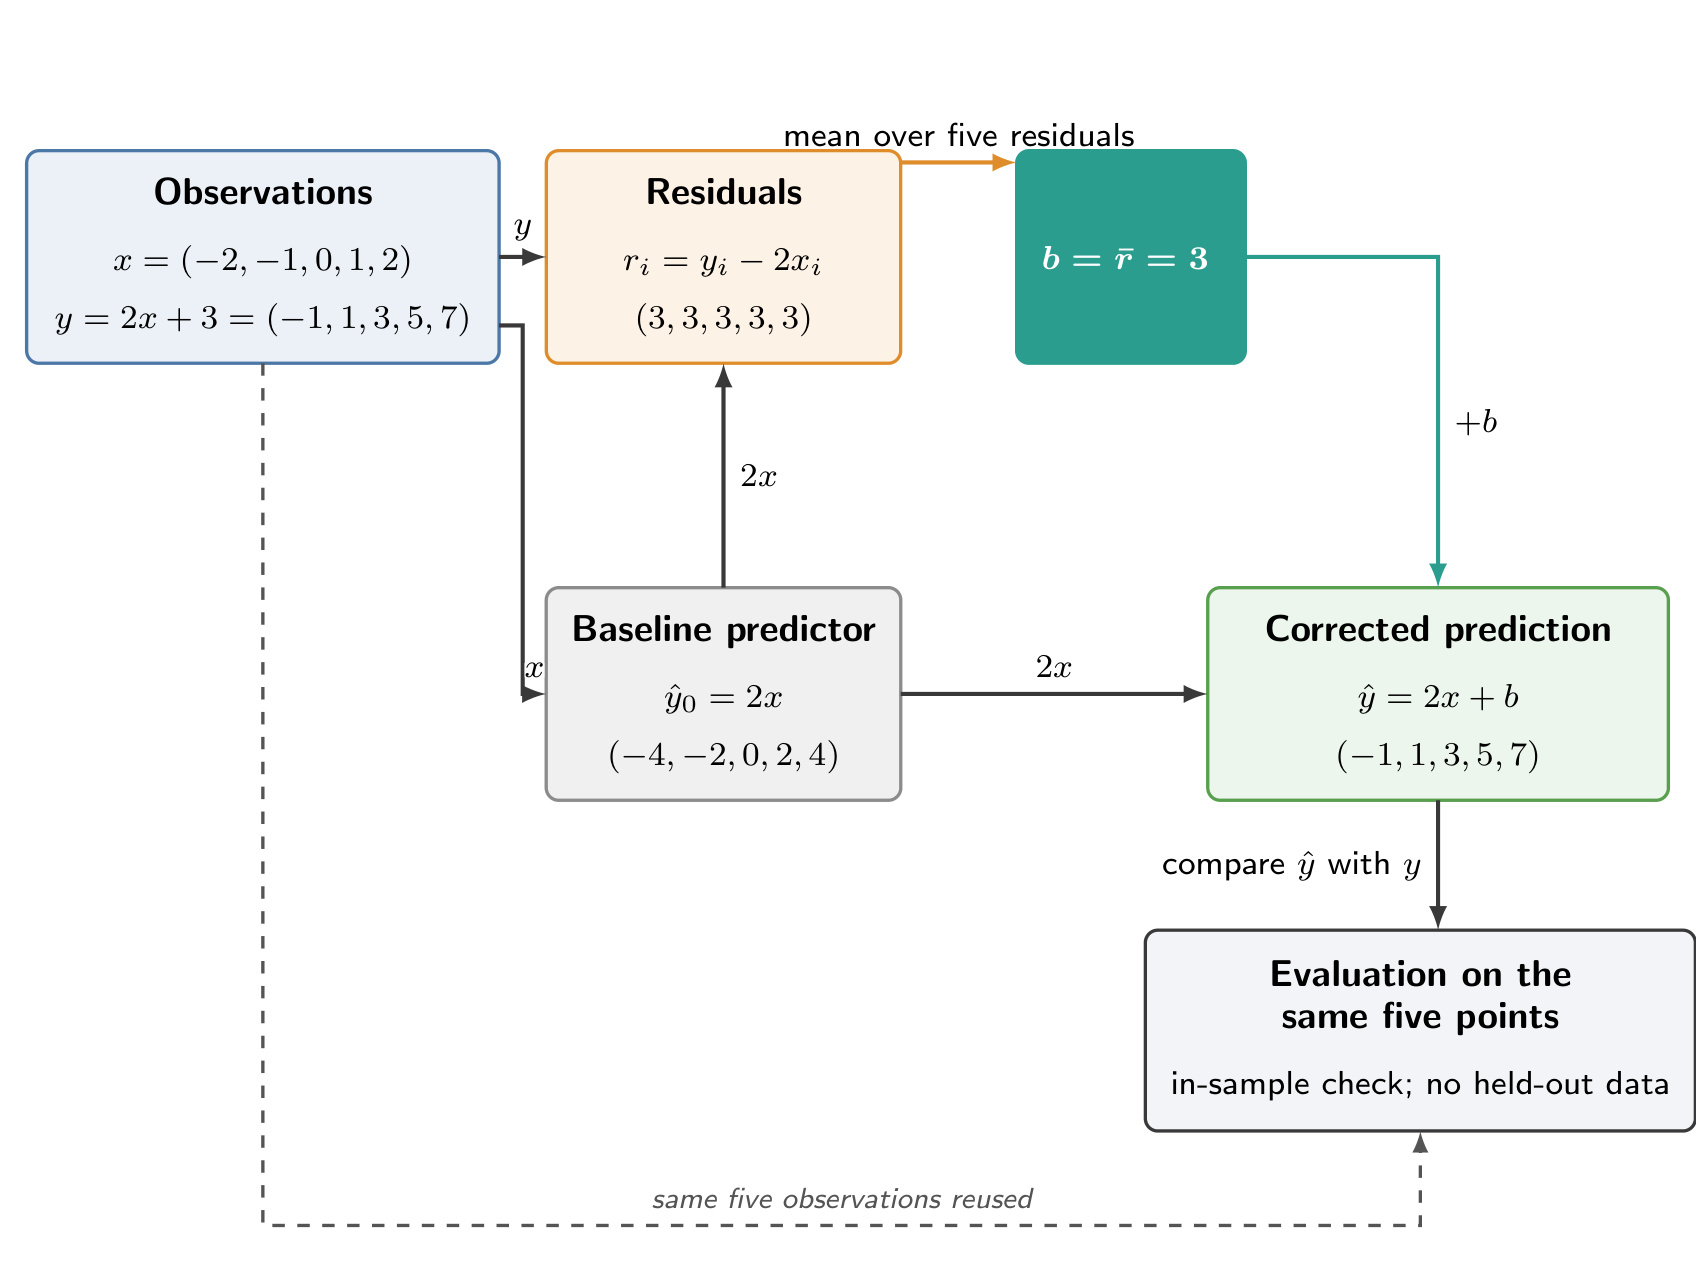
\includegraphics[width=\linewidth]{figures/fig_residual_workflow.jpg}
\caption{Residual correction and evaluation dependencies. The five residuals equal $3$, so their mean supplies $b=3$. The dashed arrow identifies the original observations reused to evaluate the corrected predictions.}
\label{fig:residual_workflow}
\end{figure}

\section{Experiments}

\subsection{Recorded Calculation and Error Definitions}

The supplied experimental record contains one deterministic calculation implemented in base R. For an added scalar $b$, define
\[
e_i(b)=y_i-(2x_i+b)=3-b.
\]
The reported summaries are
\[
\operatorname{MAE}(b)=\frac{1}{5}\sum_{i=1}^{5}|e_i(b)|,
\qquad
\operatorname{MSE}(b)=\frac{1}{5}\sum_{i=1}^{5}e_i(b)^2.
\]
Because all five differences are identical, these expressions simplify to
\[
\operatorname{MAE}(b)=|3-b|,
\qquad
\operatorname{MSE}(b)=(3-b)^2.
\]
These identities explain the recorded settings $b=0$, $1.5$, and $3$. Each setting is evaluated against the same five targets.

\subsection{Measured Errors, Visualization, and Limits}

Table~\ref{tab:recorded_errors} reproduces the complete recorded error summary. The intermediate setting $b=1.5$ has a specific instructional purpose: it removes half the common offset. Consequently, it halves both the residual magnitude and MAE, while reducing MSE to one quarter of the baseline value. This contrast makes the different scaling of absolute and squared error visible. The setting is a supplied partial correction, rather than an iteration in an optimization procedure.

\begin{table}[htbp]
\centering
\caption{Complete recorded errors. Correction and evaluation use the same five observations.}
\label{tab:recorded_errors}
\begin{tabular}{rrr}
\toprule
Added $b$ & Mean absolute error & Mean squared error \\
\midrule
0   & 3   & 9    \\
1.5 & 1.5 & 2.25 \\
3   & 0   & 0    \\
\bottomrule
\end{tabular}
\end{table}

Figure~\ref{fig:intercept_error} displays exactly the three recorded MSE pairs as discrete points. Its labels allow direct comparison with the table. The zero at $b=3$ is the arithmetic consequence of identical baseline residuals and the correction computed from them. All reported errors describe agreement on the observations entering that computation.

\begin{figure}[htbp]
\centering
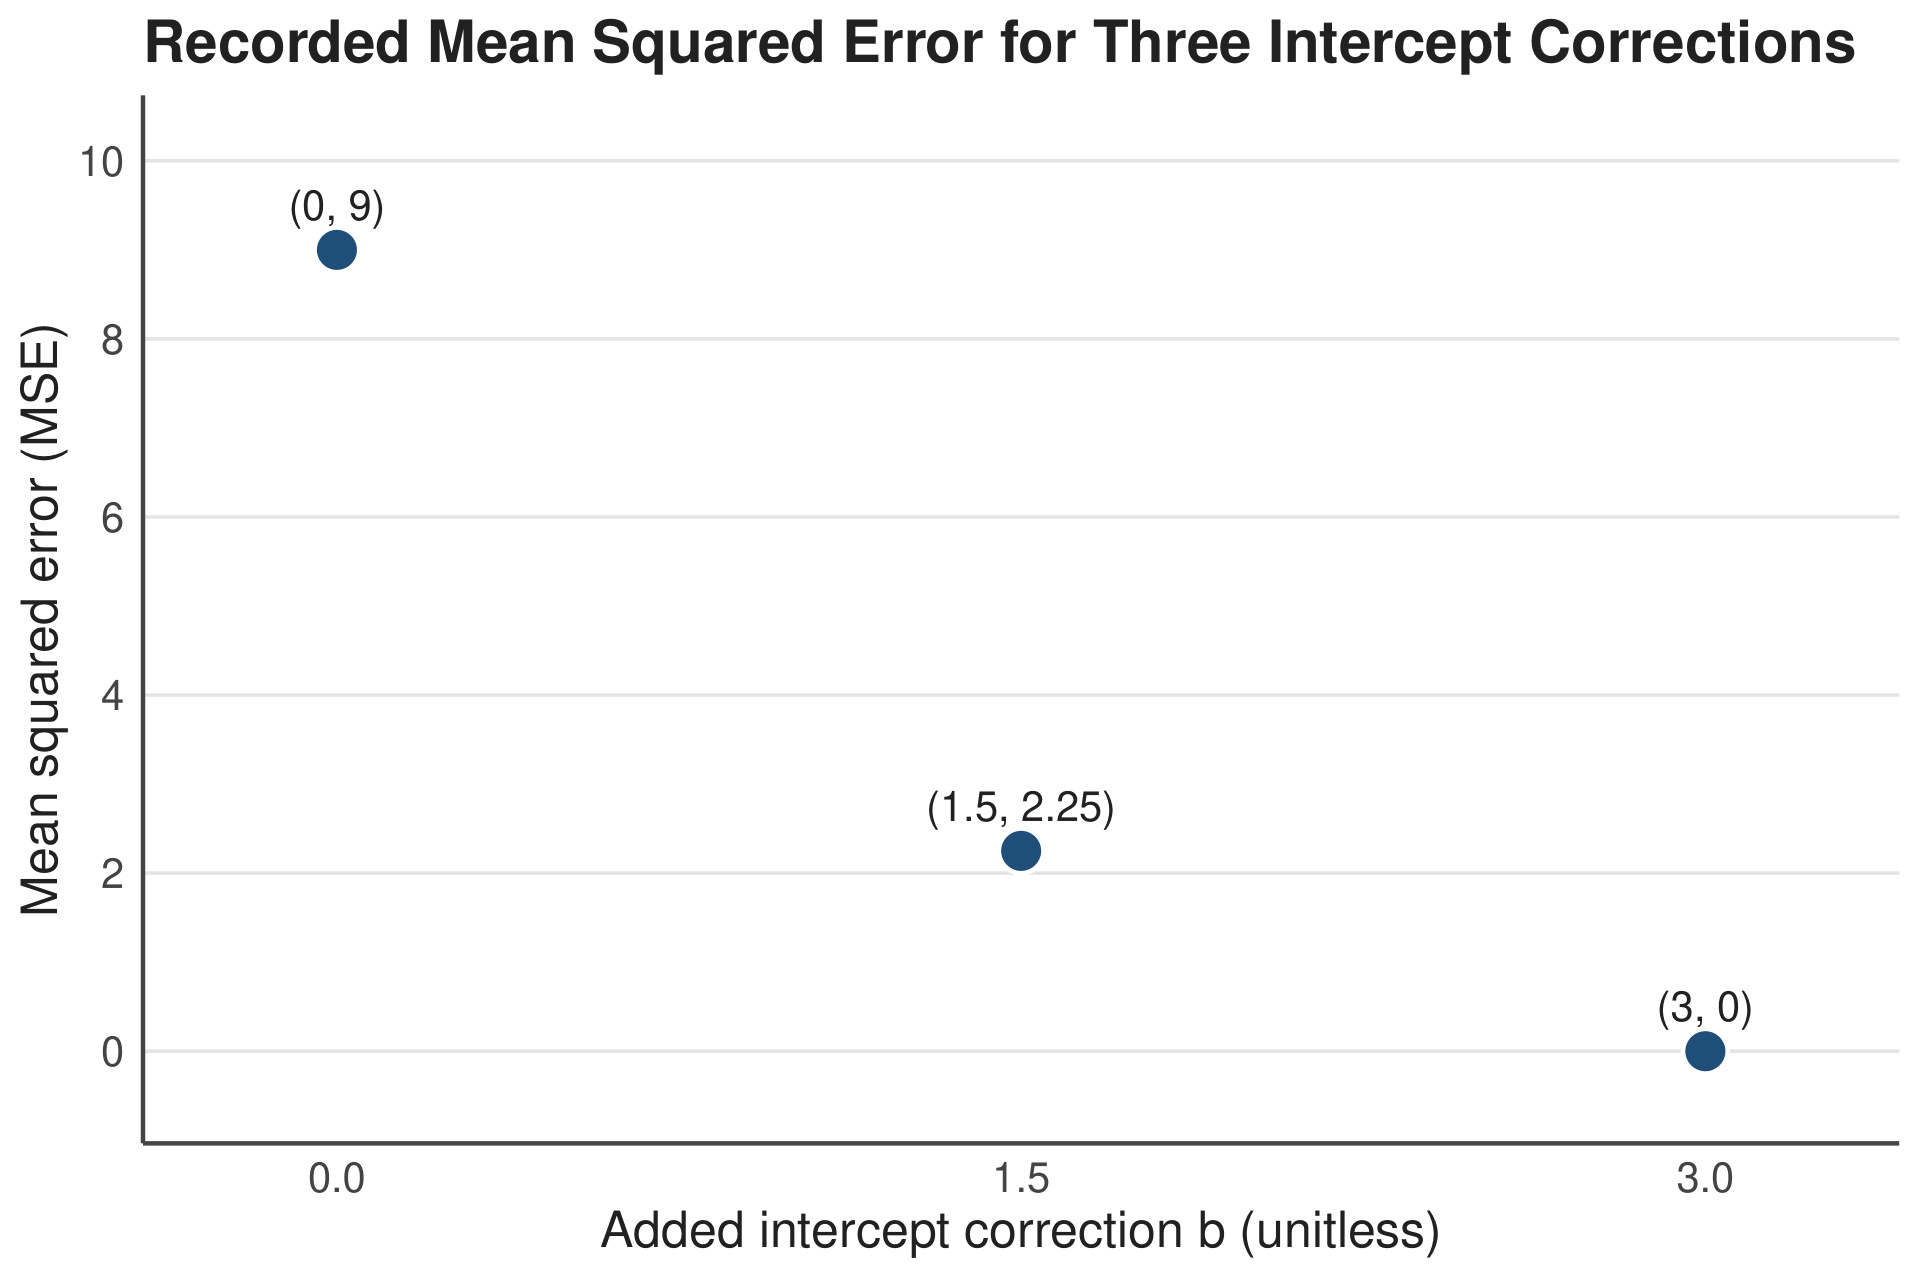
\includegraphics[width=\linewidth]{figures/fig_intercept_error.jpg}
\caption{Recorded MSE at $(b,\operatorname{MSE})=(0,9)$, $(1.5,2.25)$, and $(3,0)$. The supplied plot displays the measured pairs without interpolation.}
\label{fig:intercept_error}
\end{figure}


\section{Conclusion}

Adding the mean residual $3$ to the fixed predictor $2x$ exactly matches the five supplied targets. The intermediate correction illustrates how absolute and squared error scale differently. Together, the equations, table, plot, and dependency diagram provide a compact exercise in calculating a correction and interpreting an error through the observations used to obtain it.

\begin{thebibliography}{9}

\bibitem{Eisenhauer2003RegressionThrough}
Joseph G. Eisenhauer.
Regression through the Origin.
\emph{Teaching Statistics}, 2003.

\bibitem{Anscombe1963ExaminationAnalysis}
Francis John Anscombe and John W. Tukey.
The Examination and Analysis of Residuals.
\emph{Technometrics}, 1963.

\bibitem{Shmueli2010ExplainOr}
Galit Shmueli.
To Explain or to Predict?
\emph{Statistical Science}, 2010.

\end{thebibliography}

% PAPER_ORCHESTRA_PROVENANCE_BEGIN
\clearpage
\section*{Figure source provenance}
The files below are the exact sources that produced the embedded figure previews. Paths are relative to this manuscript's source directory. The accompanying \texttt{figure\char95{}provenance.json} records all artifact checksums.\par
\medskip\noindent\textbf{Figure~\ref{fig:intercept_error} (\texttt{fig\char95{}intercept\char95{}error.jpg}).}\par
\noindent R/ggplot2 source: \texttt{figure\char95{}code/\allowbreak{}fig\char95{}intercept\char95{}error/\allowbreak{}source.R}.\par
\noindent Source SHA256: \texttt{34ba57e5\allowbreak{}6adf6b78\allowbreak{}4bfabe24\allowbreak{}299ef6d2\allowbreak{}5ce74051\allowbreak{}70d96d8c\allowbreak{}09ada698\allowbreak{}97622aee}.\par
\noindent Rendering metadata: \texttt{figure\char95{}code/\allowbreak{}fig\char95{}intercept\char95{}error/\allowbreak{}render.json}.\par
\noindent Exact export wrapper: \texttt{figure\char95{}code/\allowbreak{}fig\char95{}intercept\char95{}error/\allowbreak{}worker.R}.\par
\noindent Wrapper SHA256: \texttt{1aedad4b\allowbreak{}1547d4b2\allowbreak{}d394cbb0\allowbreak{}239655d3\allowbreak{}667d453d\allowbreak{}d1fd0eca\allowbreak{}3e77c037\allowbreak{}e6d34892}.\par
\noindent Rendering metadata: \texttt{figure\char95{}code/\allowbreak{}fig\char95{}intercept\char95{}error/\allowbreak{}sessionInfo.txt}.\par
\medskip\noindent\textbf{Figure~\ref{fig:residual_workflow} (\texttt{fig\char95{}residual\char95{}workflow.jpg}).}\par
\noindent LaTeX/TikZ source: \texttt{figure\char95{}code/\allowbreak{}fig\char95{}residual\char95{}workflow/\allowbreak{}source.tex}.\par
\noindent Source SHA256: \texttt{e1de201d\allowbreak{}70c4a996\allowbreak{}77d8214a\allowbreak{}b33a2f9c\allowbreak{}6815b281\allowbreak{}a8c5bf20\allowbreak{}97e46cce\allowbreak{}5855da92}.\par
\noindent Rendering metadata: \texttt{figure\char95{}code/\allowbreak{}fig\char95{}residual\char95{}workflow/\allowbreak{}render.json}.\par
% PAPER_ORCHESTRA_PROVENANCE_END
\end{document}